\FloatBarrier
\section{Experimental questions: what it takes to triage}
\label{sec:eqs}

The research questions showed what happens; the experimental questions ask why, and what it means in practice. The analyses
were specified in amendments v1.1--v1.4, but their details were fixed after the primary results had been seen, and the corpus
guarantee was added and revised after external reviews. All are exploratory (Appendix~\ref{app:deviations}).

\subsection{EQ1: Does calibration error predict triage?}
\label{sec:eq1}

\textbf{Answer: no.} Calibration error is cheap to fix and says little about how well a coder ranks its errors, which is what
triage depends on.

\paragraph{Calibration is cheap to fix.} Raw calibration errors range from 0.05 to 0.33 (Table~\ref{tab:main_rq1}). A Platt or
isotonic map from confidence to accuracy, fitted per task on the calibration split, brings every signal's mean ECE over tasks
to 0.03--0.07 (Figure~\ref{fig:reliability} and Table~\ref{tab:tab07_triage_rules}, appendix). Because Platt's map is
monotone, it leaves error ranking unchanged for every decision model and verbalized signal; only for the near-saturated token
probabilities and vote shares, whose confidence carries little signal, can the fitted map flatten or even reverse it.
Temperature scaling of the full probability distribution, by contrast, is fragile here: models that output exact zeros and
ones make the fit depend on how those are floored before taking logarithms (Table~\ref{tab:tab24_temperature_floor}). With a
floor of $10^{-4}$, temperature scaling calibrated Jev well and appeared to lower the token probabilities' error ranking (Luna
0.558 to 0.489); with $10^{-12}$ it leaves Jev's ECE unchanged and raises Luna's ranking to 0.579. We therefore use Platt maps
as the recalibration yardstick and draw no conclusion from temperature scaling.

\paragraph{Low calibration error does not mean good ranking.} Clef has one of the lowest raw ECEs (0.055) but ranks errors
worse than Jev (ECE 0.120). The raw reliability curves show how the coders are miscalibrated: Jev and OpenAI Decisions are
overconfident at high confidence, Kev-27B is underconfident, and Sonnet and pplx-decider are close to calibrated. ECE here is
top-label calibration against the majority label; calibration against the distribution of human labels
\citep{baan2022stop} is a different target, which RQ2 approaches.

\paragraph{Raw probabilities mislead the overconfident coders.} Taken at face value, ``accept if confidence $\ge$0.95''
accepts 36--64\% of decisions for Jev, OpenAI Decisions, Luna and gpt-oss at 12--14\% error, and almost every decision at
24--33\% error for the token probabilities and Qwen3.5-9B's verbalized confidence. The other decision models, Haiku, Sonnet
and Qwen3.8-2.4T stay below 5\% error, mostly because few of their decisions reach 0.95 (4--31\%).

\paragraph{What it means.} A coder should not be chosen by its calibration error or by a vendor's claim of calibration.
If its probabilities will be read as probabilities, recalibrate them on the hand-coded sample; to choose between coders,
compare how well they rank errors and how much they accept at the target. A fixed rule such as ``accept $\ge$0.95'' is unsafe
for an overconfident coder.

\subsection{EQ2: Do threshold rules keep their target, and what does a guarantee cost?}
\label{sec:eq2}

\textbf{Answer: the usual rule does not; a guarantee that follows the sampling design does, at a cost.} The cost is modest on
Reddit comments and prohibitive on dialogue at our budgets.

\paragraph{The naive rule overshoots.} Over 500 random cluster re-splits per task, the naive rule's held-out error exceeds 5\%
in 47--52\% of MFRC re-splits for Jev, Clef, Clef-flash, pplx-decider and both Kev models, and in 28\% for OpenAI Decisions
(Figure~\ref{fig:rules}; per-task rates in Tables~\ref{tab:tab07b_resplits_by_task} and~\ref{tab:tab07d_resplits_guaranteed}).
The reason is simple: a threshold chosen to sit just under 5\% on calibration data lands on either side of 5\% on new data
about equally often. The LLMs' verbalized confidence overshoots less on MFRC (0--19\%), probably because its coarse confidence
levels put the threshold at a tie boundary with room to spare. On the dialogue tasks, wherever a decision model's naive rule
accepts more than 5\% of decisions, its held-out error exceeds 5\% in 37--85\% of re-splits.

\paragraph{A guarantee that ignores clustering fails.} LTT on decisions treats the eight codes of a comment, and the
utterances of a transcript, as independent. They are not: a model that misreads a comment or a stretch of conversation
can get several of its decisions wrong together. On MFRC this rule's held-out error exceeds 5\% in 5.8--11.2\% of
re-splits for every decision model, above the nominal 5\%. In simulations with calibrated confidence and errors correlated
within clusters (Table~\ref{tab:tab20_ltt_simulation}), the population risk of its threshold exceeds 5\% in 6\% of runs with
independent errors, in 14\% with strong correlation in MFRC-like clusters of eight, and in 18--31\% with dialogue-like
clusters; the error on the uncoded remainder exceeds 5\% in 10--30\% of runs.

\paragraph{The corpus guarantee holds on comments.} Corpus LTT (\S\ref{sec:rules}) never exceeds 5\% held-out error in any
re-split of any task. Because each test split is the uncoded remainder of a random split, this is a direct check of its
guarantee. LTT on i.i.d.\ clusters never exceeds it either, and in simulation both exceed 5\% in at most 0.3\% of runs, for
either target. On the frozen MFRC split, corpus LTT certifies 60--83\% of decisions for six of the seven decision models and
for Luna's, Haiku's and Sonnet's verbalized confidence, at realized test errors of 1.6--3.0\% (Table~\ref{tab:main_policies}).
It certifies nothing for OpenAI Decisions (at its highest thresholds its calibration error, 2.5--3.8\%, is too close to 5\% for
a test corrected for 16 thresholds), gpt-oss, Qwen3.8-2.4T (its subset has too few calibration comments), the token
probabilities or the agreement signals. The frozen split is one draw: over the re-splits, corpus LTT accepts on average
65--85\% of MFRC decisions for the same coders, and 64\% for gpt-oss.

\paragraph{With whole transcripts, dialogue cannot be certified.} With whole transcripts or lessons hand-coded, as in our
splits, corpus LTT certifies nothing on the dialogue tasks, for any coder, and with this procedure at our calibration sizes
nothing better was possible. The reason is the sampling unit. The test caps its bets and scales each unit by $B$, the weight
of the largest unit, so an error-free unit multiplies the evidence by at most $1+0.05\times(\text{its weight}/B)$, whatever
the order, and the evidence must reach $16/0.05=320$ (Appendix~\ref{app:ltt}). A typical transcript carries only 8--27\% of the
largest one's weight, so each adds little. On AnnoMI and TalkMoves student, even a coder that is never wrong could not be
certified, whichever transcripts were hand-coded; on TalkMoves teacher, fewer than 388 of the 444 lessons cannot suffice
(Table~\ref{tab:tab21_ltt_feasibility}).

\paragraph{Sampling utterances removes that obstacle, but the evidence is still too thin.} The corpus guarantee allows any
dependence, so single utterances drawn at random, each coded with its context, are valid units too. They weigh about the
same, and a perfect coder is then certified after a median of 139--163 hand-coded segments. Under that design, with 30\% of
segments hand-coded, the real coders still certify almost nothing (Table~\ref{tab:tab21b_utterance_sampling}): pplx-decider
and Kev-27B on AnnoMI therapist obtain a certificate in \res{ut/annomi_therapist/pplx/certs} and
\res{ut/annomi_therapist/kev27b/certs} of \res{ut/reps} re-splits (accepting about \res{ut/annomi_therapist/pplx/cond}\% and
\res{ut/annomi_therapist/kev27b/cond}\% of decisions when they do), and the other coder--task pairs in none. The confident
accepted sets supply too little evidence of $\le$5\% error. On the first re-split's roughly 430 hand-coded segments, 11 of the
44 coder--task pairs have no grid threshold at or below 5\% error against the majority label; 30 have one, but it accepts at
most 65 segments (median 9); and the three larger qualifying sets (191--227 segments, on AnnoMI therapist) sit at about 4.5\%,
too close to 5\% for a conservative test to separate. On the same re-splits the naive rule exceeds 5\% held-out error in up to
78\% of them. On dialogue, then, the binding constraints are the sampling design first and then the amount and accuracy of
confident evidence, not dependence among utterances. LTT on decisions appeared to certify 42\% (Kev-27B) and 24\% (Sonnet) on
AnnoMI therapist under the transcript design; those certificates were not valid.

\paragraph{How much hand-coding a guarantee needs.} The calibration-budget curves (Figure~\ref{fig:budget}, appendix) draw
smaller calibration sets of whole MFRC comments, keeping the test split as the remainder. Corpus LTT certifies nothing with
50, 100 or 200 hand-coded comments, and 2\% (Jev) to 78\% (Sonnet) with 400. The naive rule accepts as much with 50 comments
as with 600, but exceeds 5\% held-out error in up to 54\% of draws (pplx-decider) and still in 27\% with 400. Testing one
threshold fixed in advance (0.95) instead of the grid halves the comments a perfect coder needs (64). It certifies gpt-oss
(\res{st/oss-verbal/single}\%) but still not OpenAI Decisions, and it raises Luna's share (\res{st/luna-verbal/grid}\% to
\res{st/luna-verbal/single}\%); for the other certified coders the fixed threshold is restrictive and certifies less than the
grid, for example Jev \res{st/jev/single}\% instead of \res{st/jev/grid}\% (Table~\ref{tab:tab23_ltt_single_threshold}).

\paragraph{Thresholds do not transfer.} A threshold fitted on the other four tasks exceeds 5\% error in 52 of the 64
task--coder cells where it accepts anything (median 16\% on the dialogue tasks), and a fixed ``accept $\ge$0.95'' rule in 52 of
75. Guarantees do not travel either. Corpus LTT does not apply, because the other tasks are not a sample of the new corpus,
and LTT on i.i.d.\ clusters pooled over the other four tasks certifies nothing at all. This matches \citet{lu2026candidate},
who find that rejection thresholds of typed decision models do not carry across datasets.

\paragraph{What it means.} If the error target must hold, a researcher should hand-code a random sample from their own
corpus and use a rule whose unit matches how that sample was drawn. With this procedure, nothing is certified until about 120
error-free units of similar weight have been hand-coded, so small units (single comments or utterances, or fixed-size blocks)
are far cheaper than whole transcripts of very unequal length. Thresholds borrowed from another codebook, or fixed in advance
at a round number, should not be trusted.

\begin{figure}[tb]
  \centering
  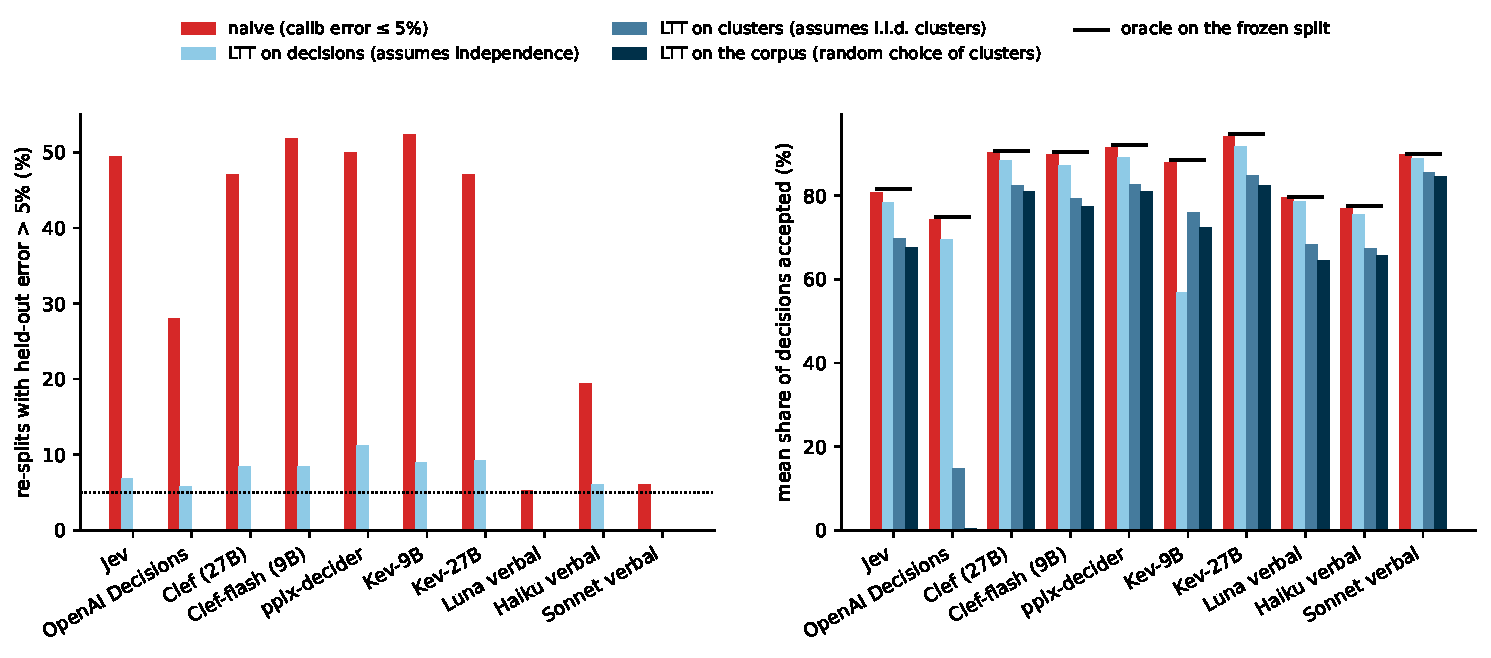
\includegraphics[width=\linewidth]{fig05_threshold_rules.pdf}
  \caption{EQ2 on MFRC, the only task where the guaranteed rules accept anything when whole clusters are hand-coded, over 500
  random cluster re-splits. Left: share of re-splits whose held-out error exceeds 5\% (dotted: 5\%). Right: mean share of test
  decisions accepted; black ticks mark the oracle on the frozen split. LTT on decisions assumes independent decisions and LTT
  on i.i.d.\ clusters independent clusters; corpus LTT assumes only that the hand-coded clusters are a random sample, visited
  in random orders.}
  \label{fig:rules}
\end{figure}

\FloatBarrier
\subsection{EQ3: Ranking or ties at the top?}
\label{sec:eq3}

\textbf{Answer: both.} For Jev and OpenAI Decisions, large blocks of decisions at the very top of the confidence scale, with
too many errors in them, limit how much can be accepted. For every coder with enough data, recalibrating per code improves
ranking, partly by using which code was predicted.

\paragraph{Large, error-prone ties at the top.} Even a threshold fitted on the test set itself (the oracle) accepts only 16\%
of Jev's decisions at $\le$5\% error, against 40\% for Sonnet. Ties at the top contribute to this (Figure~\ref{fig:blocks}).
On the dialogue tasks Jev places 8--30\% of its decisions at exactly its top confidence (1.00), and 6.5--12.3\% of those are
wrong; OpenAI Decisions behaves the same way (up to 25\% of decisions, with up to 12\% error). A threshold must accept or
reject such a tie as a whole, so for Jev none of the dialogue thresholds reaches 5\% empirical error. No other coder puts more
than 7.5\% of decisions in its top block, and Clef, Kev and pplx-decider put almost none there.

\paragraph{Per-code maps split the ties and narrow the differences.} Per-code recalibration fits a separate Platt map for each
predicted code (for MFRC, each code) on the calibration split. It splits the ties and improves error ranking for every coder
with enough calibration data: by $+$0.025 (Sonnet, Kev-27B) to $+$0.12 (Kev-9B, Qwen3.5-9B), and by
\res{pc/jev-per-code/jev-raw/dci} for Jev (Figure~\ref{fig:percode}, appendix; intervals conditional on the fitted maps). For
coders that return exact zeros and ones, the size of the gain depends on the floor applied before the logit: Jev's is
$+$0.053 with a floor of $10^{-4}$ instead of $10^{-12}$, and the token probabilities move by up to 0.024, while the other
decision models and verbalized signals change by at most 0.003 (Table~\ref{tab:tab24_temperature_floor}). Per-code maps also
narrow the differences between decision models: six of the seven land within 0.80--0.83 (OpenAI Decisions 0.77), against
0.69--0.79 raw.

\paragraph{Part of the gain is which code was predicted.} Scoring each decision only by the calibration accuracy of its
predicted code, with no confidence at all, gives 0.66--0.71 (Table~\ref{tab:tab22_category_only}); for Kev-9B this alone
beats its raw confidence (0.713 vs 0.694). Some codes are simply harder than others, and a per-code map learns that. The maps
do not make coders equivalent: oracle coverage with them still ranges from 23\% (Kev-9B) to 46\% (pplx-decider). On identical
items, Jev with per-code maps comes close to Sonnet's raw confidence, but the interval does not resolve the difference either
way (\res{pc/jev-per-code-full-calib/sonnet-verbal-raw/dci}), and it trails Sonnet with its own per-code maps
(\res{pc/jev-per-code/sonnet-verbal-per-code-own-calib/dci}; significant on MFRC, AnnoMI therapist and TalkMoves student).

\paragraph{Better ranking did not buy certified coverage at our calibration sizes.} A learned map must be fitted on clusters
that are not then used to certify it, so the maps were fitted on half of the MFRC calibration comments and certified on the
other half (304 comments). Corpus LTT then certifies 66--75\% for Clef, Clef-flash, pplx-decider and Sonnet, against
77--83\% with their raw confidence on all 608 comments, and nothing for the other coders.

\paragraph{What it means.} Per-code maps are worth fitting, since they improved ranking for every coder with enough data,
but they cost hand-coded data. They must be fitted on a pilot sample kept apart from the sample used to certify, and with a
fixed budget the better ranking can be outweighed by the smaller certification sample, so both routes should be compared
under the same budget.

\begin{figure}[tb]
  \centering
  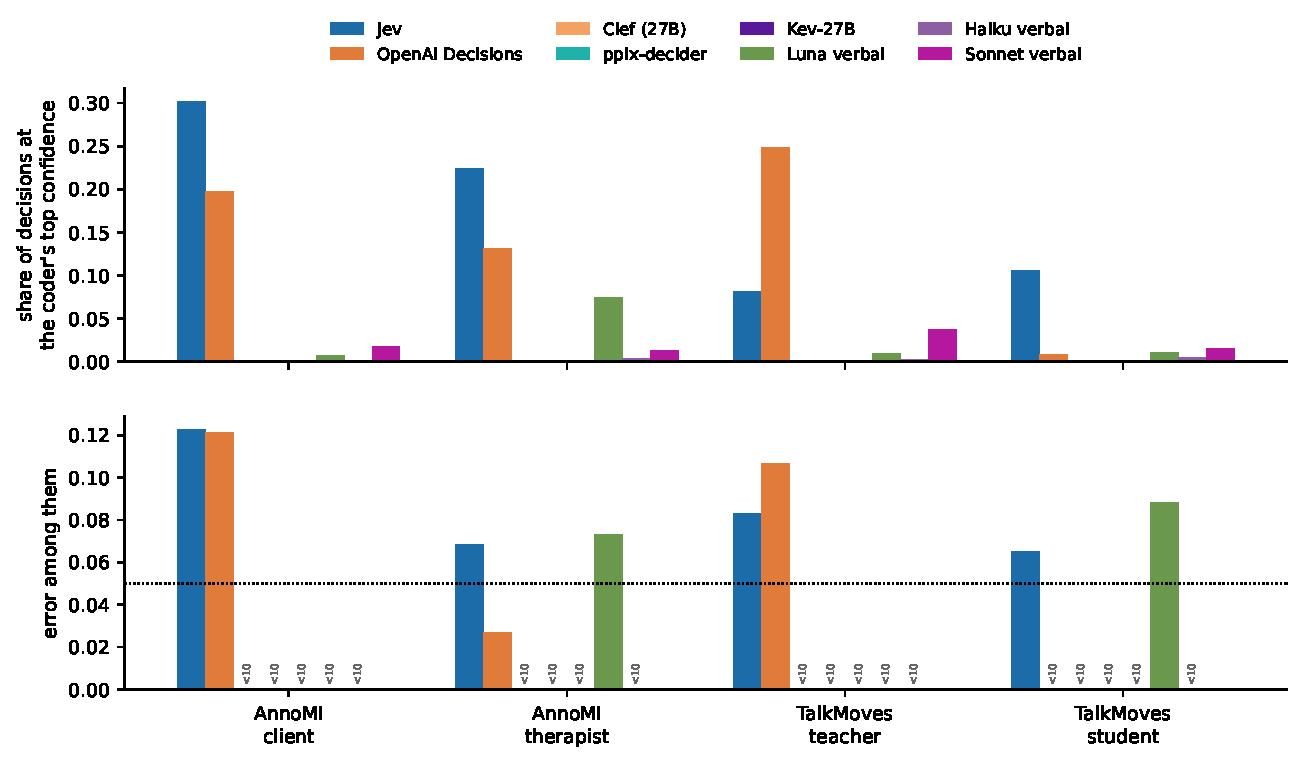
\includegraphics[width=0.85\linewidth]{fig04_top_confidence_blocks.pdf}
  \caption{EQ3: top-confidence tie blocks on the dialogue tasks. Top: share of decisions at the coder's maximum confidence.
  Bottom: error among them; blocks of fewer than 10 decisions are omitted. Above the dotted line, the top block itself exceeds
  the 5\% target.}
  \label{fig:blocks}
\end{figure}

\FloatBarrier
\subsection{EQ4: Do related 9B decision models outperform a 9B instruct model's confidence?}
\label{sec:eq4}

\begin{table}[t]
\centering
\small
\caption{EQ4: two 9B decision models built on Qwen3.5-9B vs the Qwen3.5-9B instruct model's own confidence (pooled over tasks).}
\label{tab:main_same_base}
\begin{adjustbox}{max width=\linewidth}
\begin{tabular}{llrll}
\toprule
comparison & metric & difference & 95\% CI & p (bootstrap) \\
\midrule
Clef-flash (9B) -- Qwen3.5-9B verbal & error AUROC & 0.065 & [0.048, 0.085] & <0.001 \\
Clef-flash (9B) -- Qwen3.5-9B verbal & coverage@5\% & 0.221 & [0.181, 0.297] & <0.001 \\
Clef-flash (9B) -- Qwen3.5-9B logprob & error AUROC & 0.027 & [0.004, 0.052] & 0.026 \\
Clef-flash (9B) -- Qwen3.5-9B logprob & coverage@5\% & 0.161 & [0.110, 0.211] & <0.001 \\
Kev-9B -- Qwen3.5-9B verbal & error AUROC & 0.048 & [0.030, 0.066] & <0.001 \\
Kev-9B -- Qwen3.5-9B verbal & coverage@5\% & 0.205 & [0.152, 0.280] & <0.001 \\
Kev-9B -- Qwen3.5-9B logprob & error AUROC & 0.010 & [-0.018, 0.036] & 0.512 \\
Kev-9B -- Qwen3.5-9B logprob & coverage@5\% & 0.146 & [0.079, 0.189] & <0.001 \\
Clef-flash (9B) -- Kev-9B & error AUROC & 0.018 & [-0.007, 0.043] & 0.142 \\
Clef-flash (9B) -- Kev-9B & coverage@5\% & 0.015 & [-0.043, 0.097] & 0.560 \\
\bottomrule
\end{tabular}
\end{adjustbox}
\par\smallskip\footnotesize\raggedright Coverage is the naive rule's share accepted. Kev-9B starts from the base checkpoint and Clef-flash's exact variant is unspecified, so these contrasts compare related systems with different training and read-out, not a controlled training ablation.
\end{table}


\textbf{Answer: against its verbalized confidence, yes; against its token probabilities, barely.} Clef-flash and Kev-9B are
built on Qwen3.5-9B (Kev-9B on the base checkpoint; Clef-flash on a variant Cloudflare does not specify), and we ran the
Qwen3.5-9B instruct model as a plain LLM (Table~\ref{tab:main_same_base}; pre-specified secondary). These systems differ in
training, read-out and request format, so this compares related systems, not a controlled ablation.

\paragraph{Most of the gain is over verbalized confidence, little over token probabilities.} Both decision models rank errors better than the instruct
model's verbalized confidence (\res{same_base/clef_flash/qwen-verbal/auroc/d} and \res{same_base/kev9b/qwen-verbal/auroc/d}
AUROC). Against its answer-token probabilities the gain is small: \res{same_base/clef_flash/qwen-logprob/auroc/dci} for
Clef-flash, and not significant for Kev-9B. Under the naive 5\%-target rule both accept 15--22 points more, because their
probabilities do not pile up at 1.0. Clef-flash and Kev-9B do not differ significantly.

\paragraph{Why the read-out may matter.} Our token probabilities are read after a one-sentence rationale, which likely
commits the model and contributes to the saturation. \citet{li2026llmasjev} read next-token probabilities over option
identifiers directly, without generated text, and find that a 4B base model matches decision models built on the same
backbone. Together these results suggest, as a hypothesis, that much of a decision model's advantage comes from reading out a
probability rather than from its training.

\paragraph{What it means.} A researcher with a capable open model may get much of a decision model's benefit by reading the
probabilities of the option labels directly, without a generated rationale. We did not test this; a matched-checkpoint
experiment with direct option scoring would.

\FloatBarrier
\subsection{EQ5: Which configurations give the most guaranteed automation per dollar?}
\label{sec:eq5}

\textbf{Answer: on comments, pplx-decider gives the most certified automation per inference dollar, and several
decision-model configurations come within two points of Sonnet at a fraction of its cost.} But nearly all certified decisions
are ``absent'' calls, and a person still reads most comments.

\paragraph{What each configuration certifies, and at what cost.} When whole clusters are hand-coded, as in our splits,
certificates exist only on MFRC, so we compare configurations there (Figure~\ref{fig:cost}), each at the API cost of its own
policy. Table~\ref{tab:tab08b_cascades_certified} gives the certified results and Table~\ref{tab:tab08_cascades} pooled
results under the naive rule and the oracle.
\begin{itemize}
  \item \textbf{A coder that reads nothing is not certified.} The prevalence baseline accepts 75\% of MFRC decisions at 3.6\%
  error under the naive rule, all of them ``absent''. Its scores are learned from labels, so they must be fitted on half of
  the calibration comments and certified on the other half, and corpus LTT then certifies none of its decisions.
  \item \textbf{Single decision models:} pplx-decider certifies \res{pol/pplx>human/acc}\% at
  \$\res{pol/pplx>human/usd} per 1,000 comments, Clef-flash \res{pol/clef_flash>human/acc}\% at
  \$\res{pol/clef_flash>human/usd} and Clef \res{pol/clef>human/acc}\% at \$\res{pol/clef>human/usd}; Sonnet certifies
  \res{pol/sonnet-verbal>human/acc}\% at \$\res{pol/sonnet-verbal>human/usd}.
  \item \textbf{A pplx-decider + Kev-27B agreement gate}, which accepts where both give the same label, certifies
  \res{pol/agree:pplx+kev27b>human/acc}\% at \$\res{pol/agree:pplx+kev27b>human/usd}. Its difference from Sonnet is
  \res{cas/agree:pplx+kev27b>human/sonnet-verbal>human/dci} points: not significant, which is not the same as equivalent.
  \item \textbf{Kev-27B} certifies \res{pol/kev27b>human/acc}\% at an estimated \$\res{pol/kev27b>human/usd} per 1,000
  comments, significantly more than Jev's \res{pol/jev>human/acc}\% (\res{cas/kev27b>human/jev>human/dci} points).
  \item \textbf{Chains are certified as a whole} (\S\ref{sec:rules}), and the larger joint test costs power: Kev-27B
  $\rightarrow$ Sonnet certifies \res{pol/kev27b>sonnet-verbal>human/acc}\% and Jev $\rightarrow$ Sonnet
  \res{pol/jev>sonnet-verbal>human/acc}\%, no more than Sonnet alone.
  \item \textbf{The seven-model committee} certifies \res{pol/dm_committee>human/acc}\%, slightly more than its best member
  (Clef, \res{pol/clef>human/acc}\%), at four times Clef's cost (\$\res{pol/dm_committee>human/usd}); its difference from
  Sonnet is \res{cas/dm_committee>human/sonnet-verbal>human/dci} points.
\end{itemize}

\paragraph{Accepted decisions are not reading saved, or codes found.} A comment leaves the human queue only when all eight
of its codes are accepted: under Sonnet's certified policy, \res{pol/sonnet-verbal>human/read}\% of the uncoded remainder's
comments still need a person to read at least one code, and under Jev's \res{pol/jev>human/read}\%. Counting the
\res{pol/ncal} hand-coded calibration comments as well, a person reads \res{pol/sonnet-verbal>human/readall}\% and
\res{pol/jev>human/readall}\% of all comments (Table~\ref{tab:tab08b_cascades_certified}). And 94--99.5\% of the certified
decisions say that a code does not apply: pplx-decider's certified decisions label \res{rec/pplx}\% of the codes that apply,
Sonnet's \res{rec/sonnet-verbal}\%, Jev's \res{rec/jev}\% and Kev-9B's \res{rec/kev9b}\% (Figure~\ref{fig:cost}, right;
Table~\ref{tab:main_mfrc}).

\paragraph{Inference cost is not the whole cost.} Costs are list prices for inference only. They exclude the hand-coded
calibration sample, which a guarantee requires in any case, and the human reading that remains; Kev's figure is an estimated
warm-serving cost. Human reading can dominate: per 1,000 remainder comments, Sonnet costs about \$4.49 more than pplx-decider
in inference and leaves about 75 fewer comments for a person. Assuming the same cost per human-read comment under both
policies, Sonnet has the lower combined inference-plus-reading cost on the remainder once that cost exceeds about \$0.06; this
is a sensitivity calculation, not a measured reading time.

\paragraph{What it means.} At these prices inference costs at most about \$8 per 1,000 comments, so the choice between
coders should rest on how much reading each saves and how many applying codes it finds, not only on its accepted share or its
price. Once reading is priced
in, a more accurate but costlier coder can be the cheaper policy overall.

\begin{figure}[tb]
  \centering
  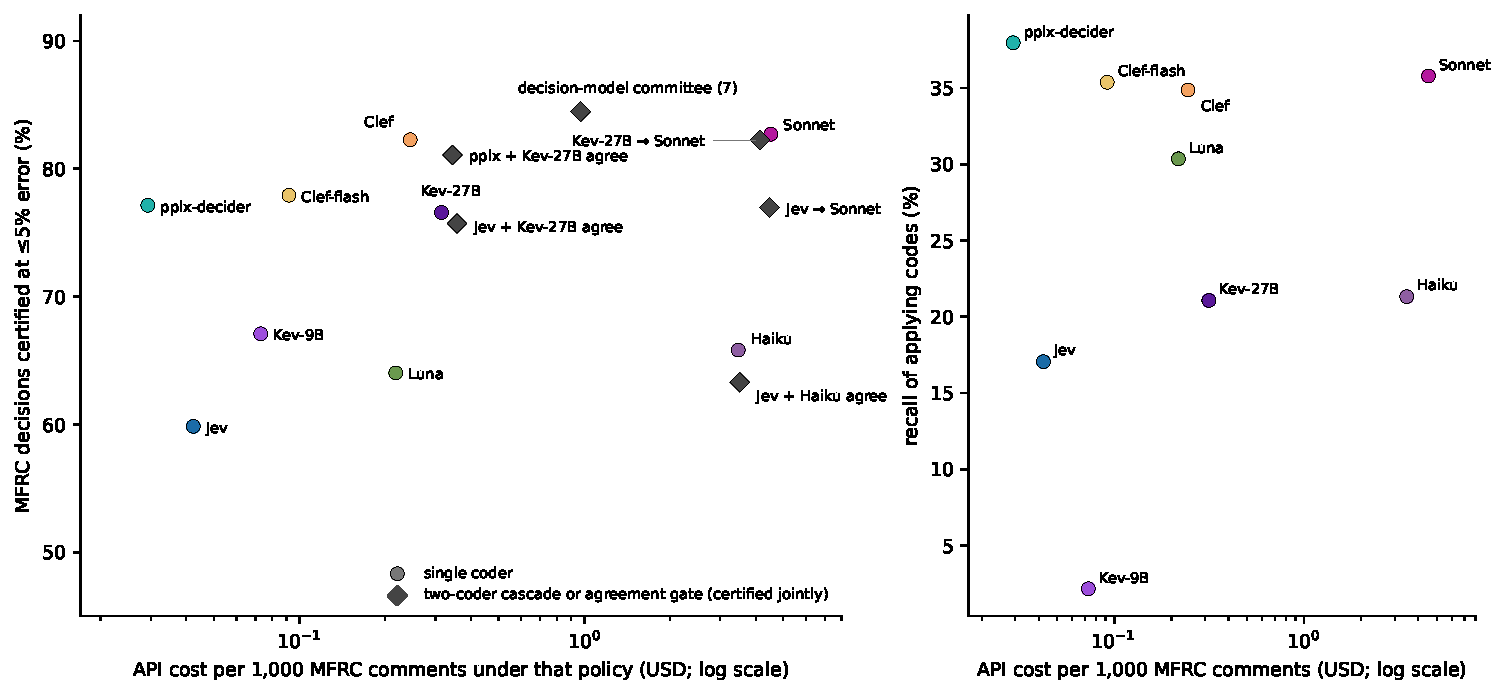
\includegraphics[width=0.9\linewidth]{fig07_cost_vs_automation.pdf}
  \caption{EQ5 on MFRC. Left: share of decisions certified at $\le$5\% error by corpus LTT vs API cost per 1,000 comments
  under the same policy (log scale); diamonds are two-coder configurations, certified jointly. Right: share of the codes that
  apply that the certified decisions label correctly. Coders that certify nothing (OpenAI Decisions, gpt-oss, the token
  probabilities, the agreement signals and the prevalence baseline) are not shown. Kev's cost is an estimated GPU serving
  cost.}
  \label{fig:cost}
\end{figure}

\FloatBarrier
\subsection{EQ6: Are the results artefacts?}
\label{sec:eq6}

\textbf{Answer: the checks bound the main threats rather than proving validity, and one of them shows that the human labels
themselves contain errors.} Table~\ref{tab:main_validity} summarizes four checks.
\begin{itemize}
  \item \textbf{Repeatability.} In the repeated requests we tested (100 test segments per task, sent twice), OpenAI Decisions,
  Clef, Clef-flash and pplx-decider returned identical outputs, and Haiku changed 0.03\% of labels. Jev changed 2.1\%, almost
  all at low confidence; Sonnet, which runs at the provider's default sampling settings, 3.3\%; and Luna 6.6\% despite
  temperature 0.
  \item \textbf{Prompt sensitivity} (v1.4). One alternative prompt, which asks for a probability for every option
  \citep{tian2023just}, does not improve the verbalized baselines: Sonnet \res{ps/sonnet-verbal/dci}, Haiku
  \res{ps/haiku-verbal/dci}. Our canonical prompt does not appear to handicap them, though one alternative cannot rule out a
  better one.
  \item \textbf{Memorization} (v1.3). Given the first half of 100 items per dataset, no model--dataset pair met the
  pre-specified completion flag, and naming the dataset never significantly increased overlap with the true continuation.
  Near-verbatim matches were rare and occurred with and without the name; they include a predictable counting sequence in a
  TalkMoves item and Du Bois quotations in Dunivin passages (Table~\ref{tab:tab15_memorization_completion}). Naming the
  dataset raised label recall in three model--task cells; a decoy name with the same description explains two as task
  framing, and the third (Luna on MFRC, $+$0.13 over the decoy) does not raise Luna's coding accuracy on those items. Decision
  models return no text and could not be probed.
  \item \textbf{Label noise and replication.} When Jev, Luna, Haiku or gpt-oss disagreed with the human label on a sampled,
  high-confidence-enriched item, adjudication sided with the coder in 55--64\% of cases (Table~\ref{tab:tab12_adjudication});
  counting only the author's verdicts (the disputed items the author adjudicated and the 12-item audit of panel-agreed
  items), it did so in 52--62\%. This echoes \citet{liu2026agreement}, but the sample cannot estimate the overall rate of
  label error. Our harness recomputes the agreement Dunivin reports for his GPT-4 runs from his released predictions
  \citep{dunivin2025scaling}, exactly, and Sonnet's mean $\kappa$ on his test set (0.679) is close to his best reported
  configuration (0.68).
\end{itemize}

\paragraph{What it means.} Some coders change a few labels when the same request is sent again, so the model version and its
outputs should be recorded with the coded data. And because the majority labels contain errors, part of every measured
``model error'' is a disagreement the model may be right about; Section~\ref{sec:discussion} returns to what this means for a
5\% target.

\begin{table}[t]
\centering
\small
\caption{EQ6: validity checks. Run-to-run flips: identical requests sent twice (100 test segments per task; 0 means identical outputs in these repeats); option-order flips: reversed and shuffled options (RQ3 arms); memorization probe with decoy-name control (amendment v1.3, deviation 14). Decision models return no text, so they could not be probed.}
\label{tab:main_validity}
\begin{adjustbox}{max width=\linewidth}
\begin{tabular}{lrrll}
\toprule
coder & \makecell[br]{run-to-run \\{} label flips} & \makecell[br]{flips under \\{} option order} & \makecell[bl]{verbatim \\{} recall \\{} (completion)} & \makecell[bl]{label recall \\{} beyond decoy} \\
\midrule
Jev & 0.021 & 0.042 & not assessed & not assessed \\
OpenAI Decisions & 0.000 & 0.096 & not assessed & not assessed \\
Clef (27B) & 0.000 & -- & not assessed & not assessed \\
Clef-flash (9B) & 0.000 & 0.006 & not assessed & not assessed \\
pplx-decider & 0.000 & 0.064 & not assessed & not assessed \\
Kev-9B & -- & 0.249 & not assessed & not assessed \\
Kev-27B & -- & -- & not assessed & not assessed \\
Luna verbal & 0.066 & 0.103 & no evidence & MFRC \\
Haiku verbal & 0.000 & -- & no evidence & no evidence \\
Sonnet verbal & 0.033 & 0.056 & no evidence & no evidence \\
gpt-oss verbal & -- & -- & no evidence & no evidence \\
Qwen3.5-9B verbal & -- & -- & no evidence & no evidence \\
Qwen3.8-2.4T verbal & -- & -- & no evidence & no evidence \\
\bottomrule
\end{tabular}
\end{adjustbox}
\par\smallskip\footnotesize\raggedright Prompt sensitivity (amendment v1.4): a verbalized-distribution prompt changes error AUROC by --0.034 [--0.056, --0.011] for Sonnet and --0.010 (n.s.) for Haiku.
\end{table}

